\documentclass[]{report}
\usepackage{mathtools}
\usepackage{amsmath}
\usepackage{amssymb}    % Math symbols such as \mathbb
\usepackage{amsthm}
\usepackage[utf8]{inputenc}
\usepackage{graphicx}
\usepackage{syntax}
%\usepackage{synttree}
\usepackage{tikz}
\usepackage{tikz-qtree}
\usetikzlibrary{positioning,shapes.geometric}
\usepackage{listings}
\usepackage[square, numbers]{natbib}
\usepackage{algorithmicx}
\usepackage{algpseudocode}
\usepackage{soul}
\sethlcolor{gray}

\lstset
{
	numbers=left,
	tabsize=2
}

% thanks to https://tex.stackexchange.com/a/53359
\algnewcommand\algorithmicassert{\textbf{assert }}
\algnewcommand\Assert[1]{\State \algorithmicassert #1}%



%https://tex.stackexchange.com/questions/9057/best-practice-for-control-flow-charts

\newcommand{\motexample}{
		\begin{figure}[!h]
		\begin{center}
		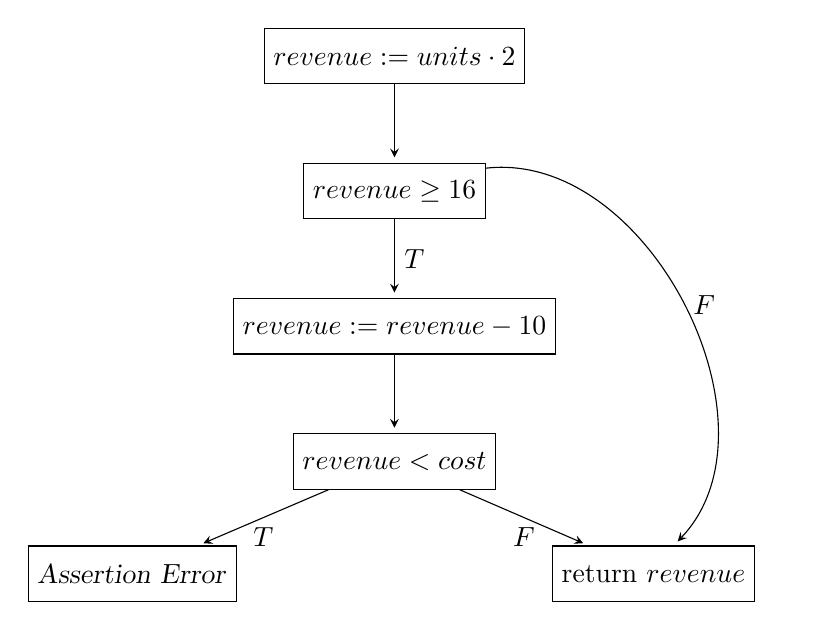
\begin{tikzpicture}[%
		->,
		shorten >=2pt,
		>=stealth,
		node distance=1cm,
		noname/.style={%
			minimum width=5em,
			minimum height=2em,
			draw,
			align=left
		}
		]
		\node[noname] (1)                                             {$revenue := units \cdot 2$};
		\node[noname] (2) [below=of 1]                                {$ revenue \geq 16$};
		\node[noname] (3) [below=of 2]						  {$revenue := revenue - 10$};
		\node[noname] (4) [below= of 3]							      {$ revenue < cost$};
		\node[noname] (5) [below left= of 4]						  {\textsl{Assertion Error}};
		\node[noname] (6) [below right= of 4]						  {return $revenue$};
		
		
		\path (1) edge             									node {} (2)
		(2) edge [bend left=70pt] 							node[right] {$F$} (6)
		(2) edge 											node[right] {$T$} (3)
		(3) edge											node {} (4)
		(4) edge 											node[right, below] {$T$} (5)
		(4) edge											node[right, below] {$F$} (6);
		\end{tikzpicture}
	\end{center}
	\caption{Control-flow graph for \textsc{ComputeRevenue}}
	\end{figure}
}

\newcommand{\sumprogram}{
	\begin{figure}[!h]
	\begin{center}
		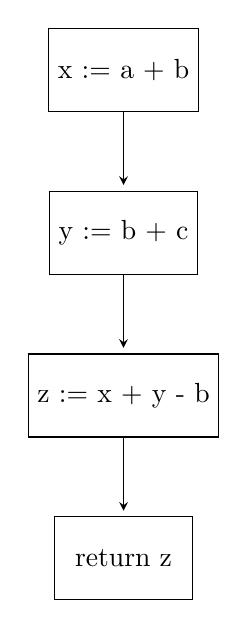
\begin{tikzpicture}[%
		->,
		shorten >=2pt,
		>=stealth,
		node distance=1cm,
		noname/.style={%
			minimum width=5em,
			minimum height=3em,
			draw
		}
		]
		\node[noname] (1)                                             {x := a + b};
		\node[noname] (2) [below=of 1]                                {y := b + c};
		\node[noname] (3) [below=of 2] 								  {z := x + y - b};
		\node[noname] (4) [below=of 3]                                {return z};
		
		\path (1) edge                   node {} (2)
		(2) edge                   node {} (3)
		(3) edge                   node {} (4);
		\end{tikzpicture}
	\end{center}
	\caption{Control-flow graph for ComputeSum}
	\end{figure}
}

\newcommand{\pow}{
	\begin{figure}[!h]
	\begin{center}
		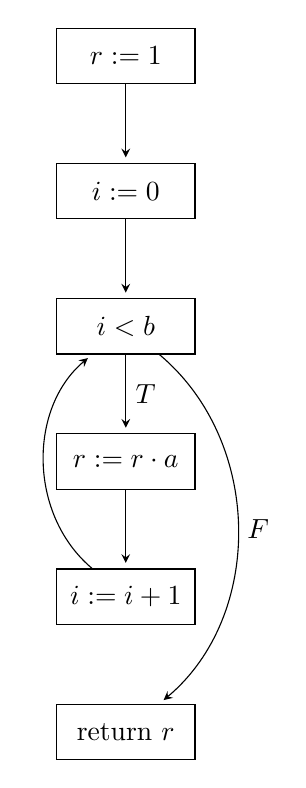
\begin{tikzpicture}[%
		->,
		shorten >=2pt,
		>=stealth,
		node distance=1cm,
		noname/.style={%
			minimum width=5em,
			minimum height=2em,
			draw
		}
		]
		\node[noname] (1)                                             {$r := 1$};
		\node[noname] (2) [below=of 1]                                {$i := 0$};
		\node[noname] (3) [below=of 2] 								  {$i < b$};
		\node[noname] (4) [below=of 3]								  {$r := r\cdot a$};
		\node[noname] (5) [below=of 4]								  {$i := i + 1$};
		\node[noname] (6) [below=of 5]								  {return $r$};
		
		
		\path (1) edge             									node {} (2)
		(2) edge                  								    node {} (3)
		(3) edge [bend left = 50pt] 								node[right] {$F$} (6)
		(3) edge                 								    node[right] {$T$} (4)
		(4) edge 												    node {} (5)
		(5) edge [bend left = 50pt]								node {} (3);
		\end{tikzpicture}
	\end{center}
	\caption{Control-flow graph for \textsc{ComputePow}}
	\end{figure}
}
\graphicspath{ {images/} }


\newcommand{\explanguage}{\textsl{SIMPL }}
\newcommand{\pc}{\emph{path-constraint} }
\newcommand{\alt}{ \ | \ }
% Title Page
\title{
	\textbf{Symbolic \& Concolic Execution}\\
	{ Symbolsk og Concolic eksekvering}\\
	\bigskip
	%{\includegraphics[scale=0.5]{ausegl_blaa.png}}	
	\large Bachelor report (15 ECTS) in Computer Science\\
	 Department of Computer Science, Aarhus University
	}
\author{Søren Baadsgaard $\cdot$ 201305284 \\
	Advisor: Magnus Madsen}
\begin{document}
\maketitle

\begin{abstract}
	Symbolic execution is a technique for systematically exploring all execution paths of a program, and for each path generate concrete input values that will execute along this path. This serves as a strong tool for testing programs, as it is often difficult to come up with a proper selection of testing inputs that cover the entire program. We describe the theory behind symbolic execution and discuss a number of limitations to the technique, such as the path-explosion problem, and the ability to decide which paths are feasible. Furthermore we describe a different technique called concolic execution, that combines concrete and symbolic execution to mitigate some of the challenges of pure symbolic execution. Finally, we demonstrate symbolic execution by describing and comparing an implementation of both a concrete and symbolic interpreter for a small toy language. 
\end{abstract}

\tableofcontents

\chapter{Introduction}
	Proper testing of programs requires a good selection of input values that cover all edge cases of the program to ensure that it behaves as expected. Choosing such a selection is often a difficult and time consuming task, and so we risk ending up with a lackluster choice of test cases, which leaves large parts of the program untested. The goal of this report is to study \emph{symbolic execution}, which is a classical technique to systematically explore all execution paths of a program and generate concrete input values that will follow these execution paths and thereby obtain test cases that properly cover the entire program. To this, the program is executed symbolically by replacing the input values with symbolic values that represents arbitrary concrete values. Whenever a conditional statement is executed, there are two potential execution paths to follow. If both paths are feasible, the execution splits into two executions, each following a different path. Each execution keeps track of the constraints that the input values must satisfy to follow that path, and from these constraints we can derive concrete input values that will execute along the same path.
\\ 
We will also study a modern approach called \emph{concolic execution} that combines concrete and symbolic execution. In this technique, the program is executed with initially random concrete input values. During the execution, we maintain both symbolic and concrete values for all variables, and whenever the execution branches, the choice of branch is registered in a list of constraints, using the symbolic values. At the end of the execution, this list of constraints is used to generate a new set of concrete input values that will cause the program to execute along a different path. This process is repeated until all execution paths have been explored.
 
\iffalse
\newpage In chapter 2 we give a motivating example, to illustrate the usefulness of symbolic execution. In chapter 3 we will describe the principles of classical symbolic execution.  
 We will also study some key challenges and limitations to this technique. 
 In chapter 4 we will describe the principles of concolic execution. We will also be comparing the two techniques to see what advantages concolic execution offer over classical symbolic execution. Finally, in chapter 5 and 6 we demonstrate the principles of symbolic execution by implementing a concrete and a symbolic interpreter for a small toy language.  
 
 \fi
	
\chapter{Motivation}
	In this chapter we will present the motivation for this project, by considering a motivating example that illustrates the usefulness of symbolic execution as a software testing technique.

\section{A motivating example}
Consider a company that sells a product with a unit price 2. If the revenue of an order is greater than or equal 16, a discount of 10 is applied. The following program that takes integer inputs $units$ and $cost$ computes the total revenue based on this pricing scheme. 


\begin{figure}[!h]
	\begin{algorithmic}[1]
		\Procedure{ComputeRevenue}{$units, cost$}
		\State $revenue := 2\cdot units$
		\If{$revenue \geq 16$}
		\State $revenue := revenue - 10$
		\Assert{$revenue \geq cost$}
		\EndIf
		\State \Return{$revenue$}
		\EndProcedure
	\end{algorithmic}
\end{figure}

\motexample

\newpage

After applying the discount, we assert that $revenue \geq cost$ since we do not wish to sell at a loss. 
We would like to know if this program ever fails due an assertion error, so we have to figure out if there exist integer inputs for which the program reaches the \textsl{Assertion Error} node in the control-flow graph. 
We might try to run the program on different input values, e.g $(units = 8, cost = 5)$, $(units = 7, cost = 10)$. These input values does not cause the program to fail, but we are still not convinced that it wont fail for some other input values.
By observing the program for some time, we realize that the input must satisfy the following two constraints to fail:

\begin{align*}
	 units \cdot 2 & \geq 16\\
	 units \cdot 2 & < cost
\end{align*}

which is the case e.g for $(units = 8, cost = 7)$. This realization was not immediately obvious, and for more complex programs, answering the same question is even more difficult. The key insight is that the conditional statements dictates which execution path the program will follow. In this report we will present \emph{symbolic execution}, which is a technique to systematically explore different execution paths and generate concrete input values that will follow these same paths. 
\chapter{Principles of symbolic execution}
	In this chapter we will cover the theory behind symbolic execution. We will start by describing what it means to \emph{symbolically} execute a program and how we deal branching. We will also explain the connection between a symbolic execution of a program, and a concrete execution. We shall restrict our focus to programs that takes integer values as input and allows us to do arithmetic operations on such values. In the end we will cover the challenges and limitations of symbolic execution that arises when these restrictions are lifted. 


\section{Symbolic executing of a program}
	
	During a normal execution of a program, input values consists of integers. During a symbolic execution we replace concrete values by symbols e.g $\alpha$ and $ \beta$, that acts as placeholders for actual integers. We will refer to symbols and arithmetic expressions over these as \emph{symbolic values}.
	 The program environment consists of variables that can reference both concrete and symbolic values. \cite{CadarSen13} \cite{King76}.
	\\
	To illustrate this, we consider the following program that takes parameters $a, b, c$ and computes the sum:
	\begin{figure}[!h]
		\begin{algorithmic}
			\Procedure{ComputeSum}{$a, b, c$}
			\State $ x := a + b$
			\State $ y := b + c$
			\State $ z := x + y - b$
			\State \Return{$z$}
			\EndProcedure
		\end{algorithmic}
	\end{figure}

	\sumprogram{}
	\newpage
	Lets consider running the program with concrete values $a = 2, b = 3$ and $c = 4$. We then get the following execution:
	First we assign $a+b = 5$ to the variable $x$. Then we assign $b + c = 7$ to the variable $y$. Next we assign $x + y - b = 9$ to variable $z$ and finally we return $z = 9$, which is indeed the sum of 2, 3 and 4. 
	\\
	Let us now run the program with symbolic input values $\alpha, \beta$ and $\gamma$ for $a, b$ and $c$ respectively. 

	
	We then get the following execution: First we assign $\alpha + \beta$ to $x$. We then assign $\beta + \gamma$ to $y$. Next we assign $(\alpha + \beta) + (\beta + \gamma) - \beta$ to $z$.Finally we return $z = \alpha + \beta + \gamma$. We can conclude that the program correctly computes the sum of $a, b$ and $c$, for any possible value of these.
	
\section{Execution paths and path constraints}
		The program that we considered in the previous section contains no conditional statements, which means it only has a single possible execution path. In general, a program with conditional statements $s_1, s_2, \ldots, s_n$ with conditions $q_1, q_2, \ldots, q_n$, will have several execution paths that are uniquely determined by the value of these conditions. In symbolic execution, we model this by introducing a \emph{path-constraint} for each execution path. The \emph{path-constraint} is a list of boolean expressions $\lbrack q_1, q_2, \ldots, q_k \rbrack$ over the symbolic values, corresponding to conditions from the conditional statements along the path. At the start of an execution, the \emph{path-constraint} only contains the expression $true$, since we have not encountered any conditional statements. to continue execution along a path, $q_1 \land \ldots \land q_k$ must be \emph{satisfiable}. To be \emph{satisfiable}, there must exist an assignment of integers to the symbols, such that the conjunction of the conditions evaluates to true. For example, $q = (2\cdot \alpha > \beta) \land (\alpha < \beta)$ is satisfiable, because we can choose $\alpha = 10$ and $\beta = 15$ in which case $q$ evaluates to \emph{true}.
		\\ 
		Whenever we reach a conditional statement with condition $q_k$, we consider the two following expressions:
		

		\begin{enumerate}
			\item $ pc \land q_k$
			\item $ pc \land \neg q_k$
		\end{enumerate}	
		where $pc$ is the conjunction of all the expressions currently contained in the \emph{path-constraint}.
		\\
		This gives a number of possible scenarios:	
		\begin{itemize}
			\item \textbf{Only the first expression is satisfiable}: Execution continues with a new \emph{path-constraint} $\lbrack q_1, q_2, \ldots, q_k \rbrack$, along the path corresponding to $q_k$ evaluating to to \emph{true}.
			\item \textbf{Only the second expression is satisfiable}:  Execution continues with a new \emph{path-constraint} $\lbrack q_1, q_2, \ldots, \neg q_k \rbrack$, along the path corresponding to $q_k$ evaluating to to \emph{false}.
			
			\item \textbf{Both expressions are satisfiable}: In this case, the execution can continue along two paths; one corresponding to the condition being \emph{false} and one being \emph{true}. At this point we \emph{fork} the execution by considering two different executions of the remaining part of the program. Both executions start with the same variable state and \emph{path-constraints} that are the same
			 up to the final element. One will have $q_k$ as the final element and the other will have $\neg q_k$. 
			These two executions will continue along different execution paths that differ from this conditional statement and onward \cite{King76}.
		\end{itemize} 
		
		To illustrate this, we consider the program from the motivating example, that takes input parameters $units$ and $costs$:
		
		\motexample{}
		\newpage
		We assign symbolic values $\alpha$ and $\beta$ to $units$ and $cost$ respectively, and get the following symbolic execution:
		
		First we assign $2\cdot \alpha$ to $revenue$. We then reach a conditional statement with condition $\alpha \cdot 2 \geq 16$. To proceed, we need to check the satisfiability of the following two expressions:
		\begin{enumerate}
			\item $true \land (\alpha \cdot 2 \geq 16)$
			\item $true \land \neg (\alpha \cdot 2 \geq 16)$.
		\end{enumerate}
		Since both these expressions are satisfiable, we need to fork. We continue execution with a new  \emph{path-constraint} $\lbrack true, (\alpha \cdot 2 \geq 16) \rbrack$, along the \emph{T} path. We also start a new execution with the same variable bindings and a \emph{path-constraint} equal to $\lbrack true, \neg (\alpha \cdot 2 \geq 16) \rbrack$. This execution will continue along the \emph{F} path, and it immediately reaches the return statement and returns $\alpha \cdot 2$.
		The first execution assigns $2\cdot \alpha - 10$ to $revenue$ and then reach another conditional statement with condition $2\cdot \alpha - 10 \geq \beta$. We consider the following expressions:
		\begin{enumerate}
			\item $true \land (\alpha \cdot 2 \geq 16) \land (((2\cdot \alpha) - 10) \geq \beta)$
			\item $true \land (\alpha \cdot 2 \geq 16) \land \neg (((2\cdot \alpha) - 10) \geq \beta)$
		\end{enumerate}
		Both of these expressions are satisfiable, so we fork again. In the end we have discovered all three possible execution paths:
		\begin{enumerate}
			\item $true \land \neg (\alpha \cdot 2 \geq 16)$
			\item $true \land (\alpha \cdot 2 \geq 16) \land (((2\cdot \alpha) - 10) \geq \beta)$
			\item $true \land (\alpha \cdot 2 \geq 16) 
			\land \neg (((2\cdot \alpha) - 10) \geq \beta)$.
		\end{enumerate}
		
		The first two \emph{path-constraints} corresponds to the two different paths that leads to the return statement, where the first one returns $2\cdot \alpha$ and the second one returns $2\cdot \alpha - 10$. Inputs that satisfy these, does not result in a crash.
		The final \emph{path-constraint} corresponds to the path that leads to the \textsl{Assertion Error}, so we can conclude that all input values that satisfy these constraints, will result in a program crash.
	
		
\section{Constraint solving}
	
	In the previous section we described how to handle programs with multiple execution paths by introducing a \emph{path-constraint} for each path, which a list of constraints on the input symbols. This system of constraints defines a class of integers that will cause the program to execute along this path. By solving the system from each \emph{path-constraint}, we obtain a member from each of class which forms a set of concrete inputs that cover all possible paths.    
	
	If we consider the motivating example again, we found three different paths, represented by the following \emph{path-constraints}:
	\begin{enumerate}
		\item $true \land \neg (\alpha \cdot 2 \geq 16)$
		\item $true \land (\alpha \cdot 2 \geq 16) \land (2\cdot \alpha - 10 \geq \beta)$
		\item $true \land (\alpha \cdot 2 \geq 16) \land \neg (2\cdot \alpha - 10 \geq \beta)$.
	\end{enumerate}
	
	By solving for $\alpha$ and $\beta$, we obtain the set of inputs $\{(7, \beta), (8,6), (8, 7)\}$, that covers all possible execution paths. Note that we have excluded a concrete value for $\beta$ in the first test case, because the \emph{path-constraint} does not depend on the value of $\beta$. 
	 
\section{Limitations and challenges of symbolic execution}
	So far we have only considered symbolic execution of programs with a small number of execution paths. Furthermore, the constraints placed on the input symbols have all been linear.
	In this section we will cover the challenges that arise when we consider more general programs.
	
	\subsection{The number of possible execution paths} 
		Since each conditional statement in a given program can result in two different execution paths, the total number of paths to be explored is potentially exponential in the number of conditional statements. 
		For this reason, the running time of the symbolic execution quickly gets out of hands if we explore all paths. 
		 The challenge gets even greater if the program contains a looping statement. In this case, the number of execution paths is infinite \cite{CadarSen13}.
		  We illustrate this by considering the following program that computes $a^b$ for integers $a$ and $b$, with symbolic values $\alpha$ and $\beta$ for $a$ and $b$:
		\begin{figure}[!h]
			\begin{algorithmic}
				\Procedure{ComputePow}{$a,b$}
				\State $r := 1$
				\State $i := 1$
				\While{$i \leq b$}
					\State $ r := r\cdot a$
					\State $ i := i + 1$
				\EndWhile
				\State \Return{$r$}
				\EndProcedure
			\end{algorithmic}
		\end{figure}
		\pow{}
		
	This program contains a \textsl{while}-statement with condition $i \leq b$. The $k'th$ time we reach this statement we will consider the following two expressions:
	\begin{enumerate}
		\item $true \land (1 \leq \beta) \land (2 \leq \beta) \land \ldots \land (k-1 \leq \beta) $
		\item $true \land (1 \leq \beta) \land (1 \leq \beta) \land \ldots \land \neg (k-1 \leq \beta) $.
	\end{enumerate}
	Both of these expressions are satisfiable, so we fork the execution. This is the case for any $k > 0$, which means that the number of possible execution paths is infinite. If we insist on exploring all paths, the symbolic execution will simply continue for ever. 
	
	\subsection{Deciding satisfiability of \emph{path-constraints}}
	A key component of symbolic execution, is deciding if a \emph{path-constraint} is satisfiable, in which case the corresponding execution path is eligible for exploration. Consider the following \emph{path-constraint} from the motivating example:
	
	\begin{equation}	
		true \land (\alpha \cdot 2 \geq 16) \land \neg (2\cdot \alpha - 10 < \beta).
	\end{equation}
	
	To decide if this is satisfiable or not, we must determine if there exist an assignment of integer values to $\alpha$ and $\beta$ such that the formula evaluates to \emph{true}. We notice that the formula is a conjunction of linear inequalities. We can assign these to variables $q_1$ and $q_2$ and get
	\begin{align}
		q_1 & = (\alpha \cdot 2 \geq 16) \\
		q_2 & = (2\cdot \alpha - 10 < \beta)
	\end{align}
	The formula would then be $true\land q_1 \land \neg q_2$,
	where $q_1$ and $q_2$ can have values \emph{true} or \emph{false} depending on whether or not the linear inequality holds for some integer values of $\alpha$ and $\beta$. The question then becomes twofold: Does there exist an assignment of \emph{true} and \emph{false} to $q_1$ and $q_2$ such that the formula evaluates to true? And if so, does this assignment lead to a system of linear inequalities that is satisfiable?
	In this example, we can assign \emph{true} to $q_1$ and \emph{false} to $q_2$, which gives the following system of linear inequalities:
	\begin{align}
		& \alpha \cdot 2 \geq 16 \\
		2  \cdot & \alpha - \beta \geq 10 
	\end{align}
	
	where we gathered the constant terms on the left hand side, and the symbols the right hand side. From the first equation we get that $\alpha \geq 8$so we select $\alpha = 8$. From the second equation we then get that $\beta \leq 6$, so we select $\beta = 6$ and this gives us a satisfying assignment for the path constraint.	
	\subsubsection{The SMT problem}
	
	The example we just gave, is an instance of the \emph{Satisfiability Modulo Theories(\textbf{SMT}) probem}. In this problem we are given a logical formula over boolean variables $q_1, q_2, \ldots, q_n$, or their negation. The task is then to decide if there exist an assignment of boolean values $true$ and $false$ to this variables, so that the formula evaluates to \emph{true}. Furthermore, each of these boolean variables represent some formula belonging to a theory. Such a theory could be the \emph{theory of Linear Integer Arithmetic(\textbf{LIA})} which we will explain shortly. If there exist an assignment that satisfies the original formula, this assignment must also be valid w.r.t the given theory. Note that the first part of this problem is simply the \emph{boolean SAT problem}, which is known to be \emph{NP-complete}, so solving this part alone takes worst-case exponential time \cite{DeMoura2011}.
	
	\subsubsection{The theory of linear integer arithmetic}
		The conditions that we have studied so far, have all had the following form:
		
		\begin{align*}
			& a_0 +  a_1 \cdot x_1 + a_2\cdot x_2 + \ldots + a_n \cdot x_n \bowtie b\\
			& where\\
			& \bowtie \in \{\leq, \geq, =\}\\
			& x_1, \ldots, x_n \in \mathbb{Z}			
		\end{align*}
		
	which is exactly the atomic expressions in the \emph{theory of linear integer arithmetic} \textbf{(LIA)}. 
	
	As an example, consider the following \emph{path-constraint} again:
	
	\begin{equation}
		true \land (\alpha \cdot 2 \geq 16) \land \neg (2\cdot \alpha - 10 < \beta).
	\end{equation}	
	We can express this as the \textbf{SMT} formula $true \land q_1 \land \neg q_2$ with $q_1 = (\alpha \cdot 2 \geq 16)$ and $q_2 = (2\cdot \alpha - \beta < 10)$, where $q_1$ and $q_2$ are atomic expressions of \textbf{LIA}.
	
	An important property of \textbf{LIA} is the fact that it is decidable. Given a formula over a number of atomic expressions, we can construct a \emph{Integer Linear Program} \textbf{(ILP)} with these expressions as constraints, and a constant objective function. This \textbf{ILP} is feasible if and only if the formula is satisfiable. We can check the feasibility of the \textbf{ILP} using the \emph{branch-and-bound} algorithm. If it is feasible, we will also get a satisfying assignment. 
	
	\subsection{Undecidable theories}
	
	We just saw that the conditions we have considered so far, are atomic expressions in the \emph{Theory of Linear Integer Arithmetic}, and that this theory is decidable. This means that we can always decide whether a given execution path is eligible for exploration.
	 
	Lets consider the following extension of the conditions that we can encounter:
	
	  
	 
	 \begin{align*}
	 	& a_0 \circ a_1 \cdot x_1 \circ a_2 \cdot x_2 \circ \ldots \circ a_n \cdot x_n \bowtie b \\
	 	& where \\
	 	& \bowtie \in  \{\leq, \geq, =\}\\
	 	& \text{\hl{$\circ \in  \{ +, \cdot \}$}}\\
	 	& x_1, \ldots, x_n \in \mathbb{Z}
	 \end{align*}
	
	This allows for non linear constraints such as $3 \cdot \alpha ^3 - 7\cdot \beta ^ 5 \leq 11$. Such expressions does not belong to \textbf{LIA}, so we are no longer guaranteed that we can decide satisfiability of the \emph{path-constraints}. In fact, they belong to the \emph{Theory of Nonlinear Integer Arithmetic} which has been shown to be an undecidable theory. %TODO cite paper that shows undecidability of NLIA
	This presents us with a major limitation of symbolic execution, since we might get stuck trying do decide the satisfiability of a \emph{path-constraint} that is not decidable.	
\chapter{Principles of concolic execution}
	In this chapter we will introduce \emph{concolic execution}, which is a technique that combines concrete and symbolic execution to explore possible execution paths. We start by describing how the technique works, and then look at the advantages that it offers compared to only using symbolic execution. As in the previous chapter, we restrict our focus to programs that takes integer values as input, and performs arithmetic operations and comparisons on these. 

\section{Concolic execution of a program}
	During a symbolic execution of a program, we replace the inputs of the program with symbols that acts as placeholders for concrete integer values. The program environment maps variables to \emph{symbolic values}, which can be integers, symbols or arithmetic expressions over these two. During a concolic execution of a program, we maintain two environments. One is a concrete environment $M_c$, which maps variables to concrete integer values. The other is a symbolic environment $M_s$ which maps variables to symbolic values. At the beginning of the execution, the concrete environment is initialized with a random integer value for each input. The symbolic environment is initialized with symbols for each input. Finally we initialize an empty path-constraint. The program is then executed both concretely and symbolically, and at the end of this execution we determine a new set of concrete input values that will cause the concrete execution to follow a different path. In the next iteration we initialize the concrete environment with these values and the program is executed concretely and symbolically again. We continue doing this until all execution paths have been explored, or some other predefined termination criteria is met \citep{Godefroid:2005:DDA:1064978.1065036}. \newpage \noindent We will now describe what we mean by executing the program both concretely and symbolically. Specifically, we will explain how we maintain our environments, how we handle conditional statements and how we generate the next set of concrete input values.
	
	\subsection{Handling the environments} 
	
	If we reach an assignment statement \textsl{v := e}, for some variable \textsl{v} and expression \textsl{e}, we evaluate \textsl{e} concretely and update our concrete environment. We also evaluate \textsl{e} symbolically and update our symbolic environment.  
	
	\subsection{Handling conditional statements}
	
	Whenever we reach a conditional statement with condition $q$, we evaluate $q$ concretely and chose a path accordingly. At the same time we evaluate $q$ symbolically and get some constraint $c$. If the concrete value of $q$ is true, we add $c$ to a path-constraint. If the concrete value of $q$ is false, we add $\neg c$ to the path constraint. This way we track which choices of paths we have made during an iteration. 
	
	\subsection{Generating input values for the next iteration}
	
	At the end of an iteration we will have a path-constraint that, for each encountered conditional statement, describes what choice of path we made. To generate the input for the next iteration, we construct a new path-constraint by negating the condition of the last conditional statement where we have not explored the other path. We then solve the constraints from this new path-constraint to obtain the next set of input values. If some input values are not constrained by this path-constraint, we keep the current concrete value for the next iteration. 

\bigskip
To illustrate concolic execution, we consider the program from the motivating example:
\motexample

\noindent First we initialize the two environments. We let 
\begin{equation*}
	M_c = \{units = 27, \ minimum = 34\}
\end{equation*}
 where 27 and 34 is chosen randomly. We let
\begin{equation*}
 	M_s = \{units =\beta, \ minimum = \alpha\}
\end{equation*}
where $\alpha$ and $\beta$ are symbols. The first statement is an assignment statement, so we get two new environments:

\begin{align*}
	M_c & = \{units = 27, \ minimum = 34, \ total = 54 \}\\
	M_s & = \{units = \alpha, \ minimum = \beta, \ total = 2\cdot \alpha \}
\end{align*}

Next, we reach an \textsl{if} statement with condition $total \geq 16$. Since $M_c(total) = 54$ we follow the \textsl{then} branch. We update the \emph{path-constraint} to $\lbrack (2\cdot \alpha \geq 16) \rbrack$. Next, we reach another \textsl{assign} statement, so we get the following environments:

\begin{align*}
	M_c & = \{units = 27, \ minimum = 34, \ total = 44 \}\\
	M_s & = \{ units = \alpha, \ minimum = \beta, \ total = 2 \cdot \alpha - 10 \}
\end{align*}

Next, we reach an \textsl{assert} statement which condition $total \geq minimum$. Since $M_c(total) = 44$ the assertion succeeds. We update the \emph{path-constraint to} $\lbrack (2\cdot \alpha \geq 16) , ((2\cdot \alpha - 10) \geq \beta) \rbrack$. Finally we return 44, which finishes one execution path.\\
To discover a new path-constraint, we make a new path-constraint by negating the final condition of the current path-constraint, so we get $\lbrack (2\cdot \alpha \geq 16), \neg ((2\cdot \alpha - 10) \geq \beta) \rbrack$. To get the next set of concrete input values, we solve the following system of constraints
\begin{align*}
	2\cdot \alpha \geq 16\\
	(2\cdot \alpha - 10) < \beta.
\end{align*}
This gives us e.g $\alpha = 8$ and $\beta = 7$. 
We then execute the program with $units = 8$ and $minimum = 7$. This execution will follow the same path until we reach the \textsl{assert}-statement. This time the execution results in an error due to the assertion being violated, and we have now explored all possible paths from the \textsl{assert}-statement. To generate the next input values, we negate the condition from the first \textsl{if}-statement and get $[\neg (2\cdot \alpha \geq 16)]$. From this we get e.g $\alpha = 5$. Since there are no constraints on the value of $\beta$, we keep the previous value.  We now execute the program with $units = 5$ and $minimum = 7$. This execution will not follow the \textsl{then} branch in the \textsl{if}-statement, so we immediately return $total$ which is 10. At this point we have explored all possible branches from each conditional statement, so we have explored all execution paths. 

\section{Handling undecidable \emph{path-constraints}} 
In the previous chapter we described how symbolic execution was limited by the ability to decide satisfiability of a path-constraint. For example, if we are executing a program with inputs $x$ and $y$ and encounter a non linear condition $ 5\cdot x - 10 \leq 3 \cdot y^3$, we might fail to decide the satisfiability of the two branches. In this case we can assume that the paths are not satisfiable and ignore them, or assume that the paths are satisfiable and continue. In the first case, we potentially miss a large number of interesting paths, and in the second case we can no longer guarantee that we only explore feasible paths.\\
The same issue may arise in concolic execution when generating the input values for the next iteration, but we are not left with same options as in symbolic execution. Since we always have access to both a concrete and a symbolic environment, we can avoid having non linear conditions in the path-constraint. Non linear conditions comes from arithmetic operations involving multiplication or division, where both operands contain symbols. In this case we can instead choose to evaluate the expression with the concrete environment \citep{Godefroid:2005:DDA:1064978.1065036}. Consider the condition $ 5\cdot x - 10 \leq 3 \cdot y^3$ again. Assume that $y$ have concrete value $2$, we then evaluate the right-hand side and get $24$. The condition then becomes $ 5\cdot x - 10 \leq 24$, which is within the theory of integer linear arithmetic, which we know we can solve. We can then decide satisfiability of the path with this more restrictive constraint. The cost of this is then the loss of completeness. If we decide to negate $5\cdot x - 10 \leq 24$ and get $5\cdot x - 10 > 24$, it is clear that solving both these constraints is not sufficient to say that all paths from the statement with condition $ 5\cdot x - 10 \leq 3 \cdot y^3$ is explored. To guarantee this we would have to check for an infinite number of possible values for $y$. So concolic execution allows us not miss as many feasible execution paths as in symbolic execution, but we are still forced forced to give up completeness if we wish to avoid exploring infeasible paths.
\chapter{Introducing the \explanguage language}
	In this chapter we will introduce \explanguage which is a small programming language which consists of top-level functions, expressions and statements.

\section{Syntax of \explanguage}

\explanguage consists of expressions and statements. Expressions evaluates to values and does not change the control flow of the program. A statement evaluates to a value and a possibly updated variable environment. They may also change the control flow of the program through conditional statements. 

\subsection{Expressions}

Expressions consists of integers$\langle I, \rangle$, booleans$\langle B \rangle$,  and variables that are referenced by identifiers$\langle Id \rangle$. Furthermore they consist of arithmetic operations and comparisons of integers. 
\begin{grammar}
	<I> ::= 0 | 1 | -1 | 2 | -2 | $\ldots$
	
	<B> ::= True | False 
	
	<Id> ::= a | b | c | $\ldots$ 
	
	<E> ::= <I> 
	\alt <B>	
	\alt <Id>
	\alt <E> + <E> | <E> - <E> | <E> * <E> | <E> / <E>
	\alt <E> \textless <E> | <E> \textgreater <E> | <E> $\leq$ <E> | <E> $\geq$ <E> | <E> $==$ <E>
\end{grammar}

\subsection{Statements}


\subsubsection{variable declaration and assignment}
Variables implicitly declared, so variable declaration and assignment are contained in the same expression:
\begin{grammar}
	<S> ::= <Id> = <Exp>
\end{grammar} 
The value of an \textsl{assignment}-statement is the value of the expression on the right-hand side.  
\subsubsection{Conditional statements}
\explanguage supports three different conditional statements, namely \textsl{if-then-else} statements, \textsl{while} statements and \textsl{assert} statements:

\begin{grammar}
	<S> ::= if <E> then <S> else <S>
	\alt while <E> do <S>
	\alt assert <E>
\end{grammar}
Where the condition must be an expression that evaluates to a boolean value. 
The value of an \textsl{if-then-else} statement is the value of the statement that ends up being evaluated, depending on the condition. In a \textsl{while} statement, we are not guaranteed that the second statement is evaluated, so we introduce a special \textsl{unit} value which will be the value of any \textsl{while} statement. An assert statement will have the \textsl{unit} value if the condition evaluates to \textsl{true}. If the condition evaluates to \textsl{false}, the execution ends with an error.

\bigskip

Finally a statement may simply be an expression, or one statement followed by another:

\begin{grammar}
	<S> ::= E
	\alt <S> <S>
\end{grammar}
 
 

\subsubsection{Functions}
\explanguage supports top-level functions that must be defined at the beginning of the program. A function declaration$\langle F \rangle$ consists of an identifier followed by a parameter list with zero or more identifiers and finally a function body which is one or more statements.

\begin{grammar}
	<F> ::= <Id> (<Id>$^{*}$) \{ <E> \}
\end{grammar}

A function call then consists of an identifier, referencing a function declaration, followed by a list of expressions which is the function arguments:

\begin{grammar}
	<E> ::= <Id> (<E>$^{*}$) 
\end{grammar}

The length of the argument list and the parameter list in the declaration must be equal. Furthermore the expressions in the argument list must evaluate to either integers or  boolean values.
The value of a function call is the value of the final statement evaluated in the function body. Since expressions only return values, functions does not have any side effects.


\subsubsection{Programs}
We finally define the syntax of a \explanguage program, which is one or more function declarations, followed by a function call. 

\begin{grammar}
	<P> ::= <F> <F>$^{*}$  <Id> (<E>$^{*}$) 
\end{grammar}









	
\chapter{Symbolic execution of \explanguage}
	In this chapter we will describe a symbolic interpreter for \explanguage. 

\section{Extension of grammar}

In order to symbolically interpret \explanguage, we must extend the grammar for the language, to include symbolic values. A symbolic value can either be a symbolic integer, a symbolic boolean or the unit value. 

\begin{grammar}
	<SV> ::= <SI> | <SB> | unit
\end{grammar}

A symbolic integer can either be a concrete integer, a symbol, or an arithmetic expression over these two.

\begin{grammar}
	<I> ::= 0 | 1 | -1 | 2 | -2 | $\ldots$
	
	<Sym> ::= a | b | c | \ldots
	
	<SI> ::= <I>
	\alt <Sym>	
	\alt <SI> + <SI> | <SI> - <SI> | <SI> * <SI> | <SI> / <SI>  
\end{grammar}

A symbolic boolean can either be \textsl{True}, \textsl{False} or a comparison of two symbolic integers. Finally, a symbolic boolean can be the negation of a symbolic boolean. This extension is needed to be able to represent the two different \emph{path-constraints} that might arise from a conditional statement.

\begin{grammar}
	<B> ::= True | False 
	
	<SB> :: = <B>
	\alt <SI> \textless <SI> | <SI> \textgreater <SI> | <SI> $\leq$ <SI> | <SI> $\geq$ <SI> | <SI> $==$ <SI>
	\alt ! <SB>
\end{grammar} 

Note that the definition of symbolic values also contain the concrete values, so we change the grammar of expressions to include symbolic values instead of just concrete values.

\begin{grammar}
	<E> ::= <SV>
\end{grammar}

\section{Path-constraints}
To represent a \pc, we implement the following classes

\begin{lstlisting}[style=simple]
case class PathConstraint(conds: List[SymbolicBool],
	ps: PathStatus)
	sealed trait PathResult
	case class Certain() extends PathResult
	case class Unknown() extends PathResult
\end{lstlisting}

This definition consists of two elements. \textsl{conds} is the list of conditions that must be met to follow the given execution path. The \textsl{PathStatus} tells us whether or not we can guarantee that the path constraint is in fact satisfiable. This is necessary because we allow for nonlinear constraints, which our \textbf{SMT} solver may fail to solve. In the case of a failure, we still explore the path but the status of the \pc will be \textsl{Unknown}.  

\section{Interpretation of expressions}
To interpret an expression, we define the following function

\begin{lstlisting}[style = simple]
 def interpExp(p: Prog,
  e: Exp, 
  env: HashMap[Id, SymbolicValue],
  pc: PathConstraint): List[ExpRes]
  
 case class ExpRes ExpRes(res: Result[SymbolicValue, String], 
 	pc: PathConstraint)
\end{lstlisting}
This definition is similar to the function from the concrete interpreter, except that the function now also takes a \pc as argument. The return type has also changed so that it now includes a \pc aswell. Further we return a list of such pairs, since expression can have several possible values depending on which execution path is followed. 

\subsection{Arithmetic and boolean expressions}
Consider an arithmetic expression 
\textsl{AExp(e1: Exp, e2: Exp, op: AOp)}. When we recursively interpret $e_1$ and $e_2$, we get two lists $L_{e_1}, L_{e_2}$ of possible results. We now need to take the cartesian $L_{e_1} \times L_{e_2}$ of the lists, and for each pair of results, we have to evaluate the arithmetic expression. 

To do this we use a \textsl{for-comprehension} which given two lists, iterate over each ordered pair of elements from the two lists.  For each pair, we \textsl{flatMap} over the two results, and if no errors are encountered, we check that both expressions evaluates to integers and compute the result.
\newpage
\begin{lstlisting}[style=simple]
	for {
		r1 <- interpExp(p, e1, env, pc)
		r2 <- interpExp(p, e2, env, r1.pc)
	} yield ExpRes(
		r1.res.flatMap(v1 => r2.res.flatMap(
		v2 => (v1, v2) match {
			case (i: IntValue, j: IntValue) => evalInts(i.v, j.v, op)
			case (i: SymbolicInt, j: SymbolicInt) => Ok(SymbolicAExp(i, j, op))
			case _ => Error("arithmetic operations on non integer values")
		})),
		r2.p
	)
\end{lstlisting}
Boolean expressions are interpreted in a similar fashion.

\subsection{Function calls}
Consider a Call expression \textsl{CallExp(id: Id, args: List[Exp])}.
To interpret this, we must first check that the function is defined and if not, we immediately return an \textsl{Error}. Otherwise, we check that the formal and actual argument list does not differ in length. Finally, if both of these things check out, we must interpret the expressions given in the \textsl{args} list, construct a local environment with the argument and interpret the statement in the function body. 
Given an argument list $[e_1, e_2, \ldots, e_n]$, we map \textsl{interpExp} on to the list, which gives a list of lists $[L_{e_1}, L_{e_2}, \ldots, L_{e_n}]$. Each list contains the possible values for the given argument, so from this we must construct all possible argument lists, which is the cartesian product over all $n$ lists $L_{e_1} \times L_{e_2} \times \ldots \times L_{e_n}$. For each possible argument list we attempt to build a local environment. If encounter an error during this process, either from the interpretation of the arguments, or from an argument having a unit value, this error will be the of function call with the given argument list. Otherwise the result will be the interpretation of the function body with the local environment. 

\section{Interpreting statements}
\chapter{Related work}
	Classical symbolic execution is introduced in \citep{King76}. The paper establishes the concept of symbolically executing a program by replacing concrete input values by symbols, and letting variables reference integer polynomials over these symbols. The concept of a \pc is also introduced as a conjunction of boolean expressions over the input symbols. These expressions are constraints placed on the input symbols that must be satisfied to execute a long the given path. Whenever the execution reaches a conditional statement, e.g an \textsl{if}-statement, the satisfiability of both execution path is checked. If both paths are satisfiable, the execution is forked into two independent executions. One execution follows the path corresponding to the condition evaluating to true, while the other follows the path corresponding to the condition evaluating to false. The paper also touches on the difficulty of deciding the satisfiability of paths, and that for most practical programs the total number of execution paths are too large to systematically explore. \citep{Godefroid:2005:DDA:1064978.1065036} presents a tool called DART(Directed Automated Random Testing), which is an instance of concolic execution. The program is executed with initially random input values. During the execution, both a concrete and a symbolic environment is maintained, and whenever the execution branches, the choice of branch is registered in a path-constraint , using the symbolic environment. At the end of an execution, the path-constraint is used to generate a new set of concrete that follow a different execution path. One of the main advantages of the DART approach is the ability to avoid getting stuck trying to decide the satisfiability of a \pc. This is achieved by substituting in concrete values whenever such undecidable contraints arises. 


\chapter{Conclusion}
	
We have demonstrated how symbolic execution, in principle, allows us to explore all possible execution paths for a program by executing the program using \emph{symbolic} values instead of concrete concrete input values. By keeping track of any constraints placed on these values by following a given execution path, we can solve these constraints to obtain concrete input values that follows the same path. This technique does have some limitations. One such limitation is the path explosion problem. The number of possible paths is potentially exponential in the number of conditional statements, and there might even be an infinite number of paths. Another limitation is the ability to decide whether a set of constraints is satisfiable or not. For some types of constraints this question is undecidable, and in this case we either have to give up exploring a large number of execution paths, or risk exploring paths that will never be executed by any concrete input values. We have also seen how this last limitation is partially mitigated by \emph{concolic execution}, where we combine concrete and symbolic execution. Here the program is executed with initially random concrete input values. During execution we maintain both symbolic and concrete values for the variables, and whenever the program branches, we keep track of which branch was chosen in a \emph{path-constraint}. This path-constraint is then used to generate the input for the next execution, which will follow a different path. By having access to both concrete and symbolic values, we can substitute symbolic values with concrete values if we ever encounter a path-constraint that we cannot solve. While this allows us to explore more paths without exploring infeasible paths, we still have to give up completeness, so the problem is not fully mitigated.

\noindent Finally we demonstrated symbolic execution by implementing both a concrete and a symbolic interpreter for a small toy language, which we compared to clearly see the differences between a concrete and symbolic execution and how the source language was extended to allow for symbolic execution. 


\appendix

\bibliographystyle{authordate3}
\bibliography{mybib}

\end{document}          
